%%%%%%%%%%%%%%%%%%%%%%%%%%%%%%%%%%%%%%%%%%%%
% En 'includes.tex' se encuentran la importación de paquetes necesarios
%%%%%%%%%%%%%%%%%%%%%%%%%%%%%%%%%%%%%%%%%%%%
%%%%%%%%%%%%%%%%%%%%%%%%%%%%%%%%%%%%%%%%%
% University Assignment Title Page 
% LaTeX Template
% Version 1.0 (27/12/12)
%
% This template has been downloaded from:
% http://www.LaTeXTemplates.com
%
% Original author:
% WikiBooks (http://en.wikibooks.org/wiki/LaTeX/Title_Creation)
%
% License: CC BY-NC-SA 3.0 (http://creativecommons.org/licenses/by-nc-sa/3.0/)
% 
% Instructions for using this template:
% This title page is capable of being compiled as is. This is not useful for 
% including it in another document. To do this, you have two options: 
%
% 1) Copy/paste everything between \begin{document} and \end{document} 
% starting at \begin{titlepage} and paste this into another LaTeX file where you 
% want your title page.
% OR
% 2) Remove everything outside the \begin{titlepage} and \end{titlepage} and 
% move this file to the same directory as the LaTeX file you wish to add it to. 
% Then add \input{./title_page_1.tex} to your LaTeX file where you want your
% title page.
%
%%%%%%%%%%%%%%%%%%%%%%%%%%%%%%%%%%%%%%%%%
%\title{Title page with logo}
%----------------------------------------------------------------------------------------
%	PACKAGES AND OTHER DOCUMENT CONFIGURATIONS
%----------------------------------------------------------------------------------------
\PassOptionsToPackage{warn}{textcomp}
\documentclass[14pt]{extarticle}
%Paquetes para idioma español y codifcación UTF8
\usepackage[spanish]{babel}
\usepackage[utf8]{inputenc}
\usepackage{csquotes}

%%% BIBLATEX
\usepackage{biblatex}
%%% BIBLIOGRAPHY
\addbibresource{references.bib}

%fuente 'fourier'
\usepackage{fourier}
%paquete para URLs
\usepackage{url}
\usepackage[hidelinks]{hyperref}
%paquete para ubicar las imágenes
\usepackage{float}
%paquete para imágenes y en dónde las tiene que buscar
\usepackage{graphicx}
\graphicspath{{images/}}
%paquete para epígrafes
\usepackage{subcaption}
%paquete para definir los márgenes de la hoja
\usepackage[left=1.5cm,right=1.5cm,top=3cm,bottom=3cm]{geometry}
%paquete para poner todos y comentarios
\usepackage[colorinlistoftodos]{todonotes}
%paquete para trabajar con código
\usepackage{listings}
%paquete para trabajar con colores y definir propios
\usepackage{color}

%paquete para el checkmark y la cruz
\usepackage{pifont}
%paquete para el signo de copyright
\usepackage{textcomp}

%paquete para que los \texttt{} no rompan el margen de la página
\usepackage[htt]{hyphenat}

\usepackage{enumerate}
%paquete para armar layouts multicolumna
\usepackage{multicol}


%Cabeceras
\usepackage{fancyhdr}
\pagestyle{fancy}
\fancyhead[L]{Administración de Redes y Seguridad, 2018}
\fancyhead[C]{}
\fancyhead[R]{UNPSJB}

\fancyfoot[R]{Luciano Serruya Aloisi}

%Comando para poner doble comillas más fácil
\newcommand{\dq}[1]{``#1''}
\newcommand{\cmark}{\ding{51}}
\newcommand{\xmark}{\ding{55}}

\definecolor{comment-green}{rgb}{0,0.5,0}
\definecolor{bg-light-gray}{HTML}{E9E9E9}
\definecolor{bg}{HTML}{D0B698}

\lstdefinestyle{bashstyle}{
    language=Bash,
    backgroundcolor=\color{bg},
    basicstyle=\ttfamily,
  	keywordstyle=\bfseries\color{white},
    stringstyle=\color{blue},
    commentstyle=\color{comment-green}\itshape,
    numberstyle=\color{gray},
    identifierstyle=\color{black},
    rulecolor=\color{gray},
    showstringspaces=false,
    escapeinside={\%*}{*)},
    morekeywords={},
    otherkeywords={},
    breaklines=true,
    frame=trbl, 
    framexleftmargin=25pt,
    numbers=left,
    xleftmargin=\parindent,
    frameround=tttt,
    captionpos=b,
    % re tirado de los pelos, pero es lo que hay
    % sacado de:
    % https://tex.stackexchange.com/questions/24528/having-problems-with-listings-and-utf-8-can-it-be-fixed
    inputencoding=utf8,
    extendedchars=true,
    literate={á}{{\'a}}1 {é}{{\'e}}1 {í}{{\'i}}1 {ó}{{\'o}}1 {Ó}{{\'O}}1 {ú}{{\'u}}1,
}



\begin{document}

%%%%%%%%%%%%%%%%%%%%%%%%%%%%%%%%%%%%%%%%%%%%
% En 'titlepage.tex' se encuentra la página de título
%%%%%%%%%%%%%%%%%%%%%%%%%%%%%%%%%%%%%%%%%%%%
\begin{titlepage}

    \newcommand{\HRule}{\rule{\linewidth}{0.5mm}} % Defines a new command for the horizontal lines, change thickness here

    \center % Center everything on the page
     
    %----------------------------------------------------------------------------------------
    %	HEADING SECTIONS
    %----------------------------------------------------------------------------------------

    \textsc{\LARGE UNPSJB}\\[1cm] % Name of your university/college
    \textsc{\Large Licenciatura en Sistemas OPGCPI}\\[0.5cm] % Major heading such as course name
    \textsc{\large Administración de Redes y Seguridad}\\[0.5cm] % Minor heading such as course title

    %----------------------------------------------------------------------------------------
    %	TITLE SECTION
    %----------------------------------------------------------------------------------------

    \HRule \\[0.4cm]
    {\huge \bfseries Trabajo Práctico 1}\\[0.4cm] % Title of your document
    {\large \bfseries Concientización}\\[0.4cm] % Title of your document
    \HRule \\[1.5cm]
     
    %----------------------------------------------------------------------------------------
    %	AUTHOR SECTION
    %----------------------------------------------------------------------------------------


    \begin{minipage}[l]{0.5\textwidth}
        \begin{flushleft}
            \textbf{\textsf{Cátedra}}\\
            \large Lic. Bruno Damián Zappellini\\ 
            \linespread{4}
            \end{flushleft}
    \end{minipage}
    \begin{minipage}[l]{0.4\textwidth}
        \begin{flushright}
            \textbf{\textsf{Integrantes:}}\\
            \linespread{1}
            \large Luciano Serruya Aloisi\\
        \end{flushright}
    \end{minipage}\\[1.5cm]

    % If you don't want a supervisor, uncomment the two lines below and remove the section above
    %\Large \emph{Author:}\\
    %John \textsc{Smith}\\[3cm] % Your name

    %----------------------------------------------------------------------------------------
    %	DATE SECTION
    %----------------------------------------------------------------------------------------

    {\large \today}\\[1cm] % Date, change the \today to a set date if you want to be precise

    %----------------------------------------------------------------------------------------
    %	LOGO SECTION
    %----------------------------------------------------------------------------------------

    
\includegraphics[scale=1]{logoUnpsjb.png}\\[0.5cm] % Include a department/university logo - this will require the graphicx package
     
    %----------------------------------------------------------------------------------------

    % \vfill % Fill the rest of the page with whitespace

\end{titlepage}


%%%%%%%%%%%%%%%%%%%%%%%%%%%%%%%%%%%%%%%%%%%%
% INDICE
%%%%%%%%%%%%%%%%%%%%%%%%%%%%%%%%%%%%%%%%%%%%
\clearpage
\tableofcontents
\clearpage 

\lstset{style=bashstyle}

\section{Introducción}

El presente trabajo de investigación se tratará sobre la \emph{criptomoneda}\footnote{Moneda digital o virtual diseñada para funcionar como medio de intercambio. Utiliza la criptografía para asegurar y verificar transacciones \autocite{CointelegraphBitcoin}} bitcoin, haciendo foco principlamente sobre los sistemas de criptografía que utiliza. 

La primer parte explicará de manera amplia lo que es la criptografía, y hará hincapié en los tipos de criptografía que implementa el protocolo Bitcoin. También incluirá las funciones de \emph{hash} que utiliza, y los algoritmos de codificación. Luego, desarrollará sobre las transacciones en Bitcoin (su ciclo de vida y cómo son validadas), siempre incluyendo los elementos de criptografía utilizados.

Por último, el trabajo explicará brevemente la red de comunicaciones en la que corre el protocolo Bitcoin -\emph{blockchain}- y cómo es la inclusión de nuevos datos a la red (minería de bloques). También otro tema muy importante en el protocolo y con mucha presencia de la criptografía que son las \emph{billeteras} de bitcoin y cómo se generan. 

\subsection{Qué es Bitcoin}

Bitcoin es la primer aplicación de la tecnología blockchain. Comenzó una revolución con la introducción de la primer moneda digital totalmente descentralizada, y demostró ser extremadamente segura y estable \autocite{MasteringBlockchainBitcoin}

El \emph{paper} titulado \emph{Bitcoin: A Peer-to-Peer Electronic Cash System}, escrito por \emph{Satoshi Nakamoto}, introduce la idea de un \emph{dinero digital} que no necesita un banco intermediario para transferir pagos entre pares.

Bitcoin se puede definir de varias maneras; es un \textbf{protocolo}, es una \textbf{moneda digital}, y es una \textbf{plataforma}. Es una combinación de redes \emph{peer-to-peer}, protocolos de comunicación, y software que facilitan la creación y uso de la moneda digital llamada bitcoin. Nótese que Bitcoin con \emph{B} mayúscula se refiere al protocolo, mientras que bitcoin con \emph{b} minúscula se refiere a la moneda. Los nodos en la red \emph{peer-to-peer} se comunican utilizando el protocolo Bitcoin \autocite{MasteringBlockchainBitcoin}.  

Una de las principales ventajas de bitcoin frente a otros proyectos para generar un dinero electrónico, es la forma en la que soluciona el \textbf{problema del doble gasto}\footnote{Situación en la que se realizan dos o más transacciones con un mismo dinero}.

\subsection{Criptografía}

La criptografía es un área de estudio que consiste de varios esquemas y técnicas para transformar un mensaje en texto plano en un mensaje cifrado; este proceso de transformación se conoce como \textbf{encripción}, mientras que el proceso de conseguir el mensaje original a partir del cifrado se llama \textbf{desencripción} \autocite{StallingsCryptography}

\subsubsection{Simétrica}

La criptograía simétrica (o \emph{encripción de clave secreta}) encripta un mensaje utilizando \textbf{una única llave} - la misma llave que encripta el mensaje desencripta el mensaje cifrado para obtener de nuevo el original. 

\begin{figure}[H]
    \centering
    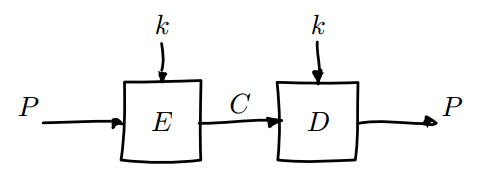
\includegraphics[width=0.8\linewidth]{images/van-houvten-simetrico.png}
    \caption*{Cifrado y descifrado simétrico (\texttt{P} representa el texto plano, \texttt{C} el mensaje cifrado, \texttt{E} y \texttt{D} las funciones de cifrado/descifrado respectivamente, y \texttt{k} la clave secreta) \autocite{VanhouvtenBlockCiphers}}
\end{figure}

Los algoritmos de encriptación simétricos pueden trabajar con \emph{bloques} (encriptando bloques de un mismo tamaño), o con \emph{flujos} (encriptando flujos de datos, pueden ser flujos de 1 bit).  

Este tipo de encriptación es muy performante y no incrementa el tamaño del mensaje, pero introduce una vulnerabilidad al tener que compartir la clave secreta entre las partes que se están queriendo comunicar.

\subsubsection{Asimétrica}

La encriptación asimétrica (o \emph{encripción de clave pública}), a diferencia de la simétrica que utiliza una única clave, necesita de dos llaves para funcionar: una \textbf{una privada} y \textbf{una pública}.  

Este sistema de encriptación se basa en que se utiliza una clave para encriptar el mensaje, y otra clave (diferente de la primera, pero relacionada) para desencriptar el mensaje. Su característica principal se trata de que se computacionalmente inviable determinar la clave de desencripción solamente sabiendo el algoritmo de cifrado y la clave de encripción \autocite{StallingsPublicKeyPrinciples}.

Teniendo este par de claves, se puede operar de dos modos distintos:

\begin{itemize}
    \item Modo encripción: el emisor encripta el mensaje con la clave pública del receptor, de modo que sólo el receptor sea capaz que de desencriptar el mensaje (utilizando su clave privada)
    \item Modo autenticación: el emisor encripta el mensaje (o un \emph{digesto} del mensaje) con su clave privada y los anexa al mensaje. El receptor desencripta este anexo con la clave pública del emisor, y compara el anexo desencriptado con el mensaje (o el digesto pudo generar el receptor). Si son iguales, entonces se garantiza que el mensaje fue enviado por el emisor, y que no fue alterado en el camino
\end{itemize}

Claramente este tipo de encripción genera mayor seguridad en la comunicación, debido a que las claves para desencriptar los mensajes no se deben intercambiar entre las partes previamente a comenzar la comunicación (son privadas a cada cliente y no deben ser reveladas). Sin embargo, aumentan el tamaño del mensaje y no son algoritmos tan performantes como los simétricos.

\subsubsection*{Criptografía de curva elíptica}

Uno de los primeros algoritmos de clave pública que se diseñaron fue \emph{RSA}\footnote{Nombrado así por las iniciales de sus creadores (\emph{Rivest–Shamir–Adleman})}, que se traba de generar pares de claves privada/pública en base a la teoría de números primos. Para brindar mayor seguridad, el algoritmo precisa números cada vez más grandes; debido a que conseguir números primos resulta una tarea muy costosa para las computadoras, este tipo de algoritmos no es ideal para dispositivos con poco poder de cómputo o poca batería

En 1985, \emph{Neal Koblitz} y Victor Miller plantearon algoritmos de criptografía basados en \emph{curvas elípticas} \autocite{MediumECC}. Una curva elíptica está definida por el conjunto de valores que genera la siguiente función \autocite{CorbelliniECC}:

\[ y^2 = x^3 + ax + b\]

Una característica muy interesante que tienen este tipo de curvas (y que es en la que se basa el algoritmo), es que si una recta intersecta dos puntos de la curva, también intersectará un tercero

\begin{multicols}{2}

    \begin{figure}[H]
        \centering
        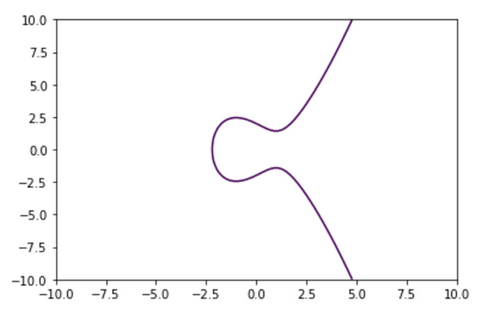
\includegraphics[width=\linewidth]{images/hackernoon-ecc-1.png}
        \caption*{Curva elíptica \autocite{HackernoonECC}}
    \end{figure}

    \begin{figure}[H]
        \centering
        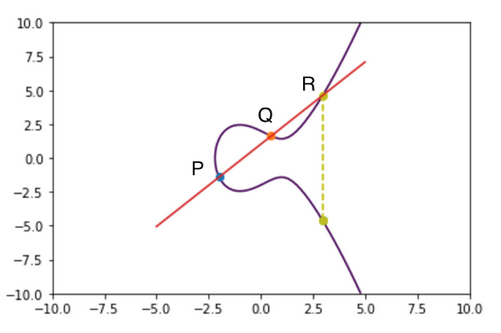
\includegraphics[width=\linewidth]{images/hackernoon-ecc-2.png}
        \caption*{Recta que atraviesa los puntos \texttt{(P, Q)}; también atraviesa el punto \texttt{(R)} \autocite{HackernoonECC}}
    \end{figure}
    
\end{multicols}

Nótese también que la curva es simétrica con respecto al eje \emph{Y}.

Sin entrar en más detalles de la criptografía de curva elíptica, el par de claves privada/pública se genera gracias a esta característica de intersección de puntos.

\subsection{Funciones de \emph{hash}}

Otro elemento de la criptografía muy importante para Bitcoin son las funciones de \emph{hash} (la mayor carga de trabajo del protocolo se trata de calcular \emph{hashes}).

Las funciones \emph{hash} se tratan de funciones que toman una entrada de largo variable y lo convierten en un valor de largo fijo, también conocido como \dq{digesto} \autocite{VanhouvtenHashIntro} 

\subsubsection{\emph{SHA256}}

La familia SHA (\emph{Secure Hash Algorithm}, Algoritmo de \emph{Hash} Seguro) es un sistema de funciones \emph{hash} criptográficas relacionadas de la Agencia de Seguridad Nacional de los Estados Unidos (NSA) y publicadas por el National Institute of Standards and Technology (NIST) \autocite{WikipediaSHA}. SHA256 es un \emph{hash} de 64 dígitos hexadecimales \emph{casi único} de un tamaño fijo de 256 bits (32 bytes) \autocite{OroYFinanzasSHA}. 

\subsubsection{\emph{RIPEMD160}}

RIPEMD160 (acrónimo de \emph{RACE Integrity Primitives Evaluation Message Digest}, primitivas de integridad del resumen del mensaje) es un algoritmo del resumen del mensaje de 160 bits desarrollado en Europa por \emph{Hans Dobbertin}, \emph{Antoon Bosselaers} y \emph{Bart Preneel} \autocite{WikipediaRIPEMD160}.

RIPEMD160 fue diseñado en la comunidad académica abierta, en contraste con el algoritmo SHA-1, diseñado por la Agencia de Seguridad Nacional estadounidense (\emph{NSA}). Por otra parte, RIPEMD160 es un diseño menos popular y no está tan estudiado com las funciones SHA. Los \emph{hashes} de 160 bits RIPEMD (también llamados resúmenes RIPE del mensaje) se representan típicamente como números en código hexadecimal de 40 dígitos \autocite{OroYFinanzasRIPEMD160}.


\subsection{Codificaciones}

Los algoritmos de codificación \emph{binario-a-texto} transforman una secuencia de datos binarios a una secuencia de caracteres imprimibles. Estas codificaciones son necesarias cuando el canal de transmisión no acepta datos binarios \autocite{WikipediaEncoding} 

\subsubsection{\emph{Base58Check}}

El algoritmo de \emph{Base58Check} es una versión modificada del \emph{Base58}, y sirve para codificar arreglos de bytes en cadenas legibles para un humano \autocite{WikipediaBase58Check}  

\section{Transacciones}
\subsection{Ciclo de vida}
\subsection{Verificación de una transacción}

\section{\emph{Blockchain}}
\subsection{Estructura de un bloque}

\section{Minería de bloques}
\subsection{Prueba de trabajo}

\section{Billeteras}






%%%%%%%%%%%%%%%%%%%%%%%%%%%%%%%%%%%%%%%%%%%%
% FIN DOCUMENTO, AHORA REFERENCIAS
%%%%%%%%%%%%%%%%%%%%%%%%%%%%%%%%%%%%%%%%%%%%
\clearpage
\printbibliography

\end{document}
